\documentclass[tikz=true]{standalone}
\begin{document}
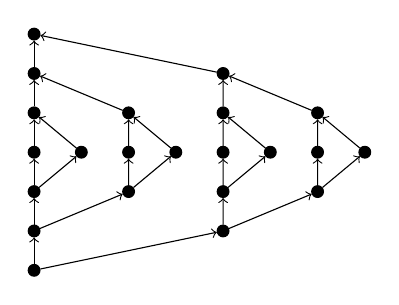
\begin{tikzpicture}
  % Tree
  \begin{scope}[xscale=0.6, yscale=0.50, every node/.style={draw, shape=circle, fill=black, inner sep=1.5pt}]
    \node (n00) at (0,0) {};
    \node (n01) at (0,1) {};
    \node (n02) at (0,2) {};
    \node (n03) at (0,3) {};
    \node (n04) at (0,4) {};
    \node (n05) at (0,5) {};
    \node (n06) at (0,6) {};

    \node (n13) at (1,3) {};

    \node (n22) at (2,2) {};
    \node (n23) at (2,3) {};
    \node (n24) at (2,4) {};

    \node (n33) at (3,3) {};

    \node (n41) at (4,1) {};
    \node (n42) at (4,2) {};
    \node (n43) at (4,3) {};
    \node (n44) at (4,4) {};
    \node (n45) at (4,5) {};

    \node (n53) at (5,3) {};

    \node (n62) at (6,2) {};
    \node (n63) at (6,3) {};
    \node (n64) at (6,4) {};

    \node (n73) at (7,3) {};

    \draw[->] (n00) edge (n01);
    \draw[->] (n00) edge (n41);

    \draw[->] (n01) edge (n02);
    \draw[->] (n01) edge (n22);

    \draw[->] (n41) edge (n42);
    \draw[->] (n41) edge (n62);

    \draw[->] (n02) edge (n03);
    \draw[->] (n02) edge (n13);

    \draw[->] (n22) edge (n23);
    \draw[->] (n22) edge (n33);

    \draw[->] (n42) edge (n43);
    \draw[->] (n42) edge (n53);

    \draw[->] (n62) edge (n63);
    \draw[->] (n62) edge (n73);

    \draw[->] (n03) edge (n04);
    \draw[->] (n13) edge (n04);

    \draw[->] (n23) edge (n24);
    \draw[->] (n33) edge (n24);

    \draw[->] (n43) edge (n44);
    \draw[->] (n53) edge (n44);

    \draw[->] (n63) edge (n64);
    \draw[->] (n73) edge (n64);

    \draw[->] (n04) edge (n05);
    \draw[->] (n24) edge (n05);

    \draw[->] (n44) edge (n45);
    \draw[->] (n64) edge (n45);

    \draw[->] (n05) edge (n06);
    \draw[->] (n45) edge (n06);

  \end{scope}
\end{tikzpicture}
\end{document}
